\chapter{Analysis}
A lot of considerations has gone into the development process of the application. The following chapter explains the considerations with the most impact on the application.

\section{Comparison}
It's been discussed if it should be possible to compare data from multiple wind farms at the same time, and how it should be done if that was the case.

One of the ideas was to let single click on a windmill put it in a `selected' state and a double click on a windmill would trigger the comparison view between all the windmills in the `selected' state.

The comparison view was also discussed to be either one chart, like the one implemented, but with all the data represented with different colors for each wind farm.
Another way of viewing them was to have multiple small draggable windows, each one representing a wind farm. This would allow browsing the data for each wind farm independent of each other, but also make it annoying when wanting to compare the same time and having to manually move forth or back in time on each window.

We chose to drop comparison because we fell short of time, but the above ideas could be used to develop some sort of comparison of data from multiple sources at the same time.

\section{Radar annotation}
In the final stages of the application, it was discussed if radars should have its name and/or time stamp for the current radar image shown.

Figure \ref{fig:mock_up_inactive_radar} and \ref{fig:mock_up_active_radar} shows the mock ups for the radar in both inactive and active state.
\begin{figure}[htbp]
  \begin{minipage}[b]{0.5\linewidth}
    \centering
    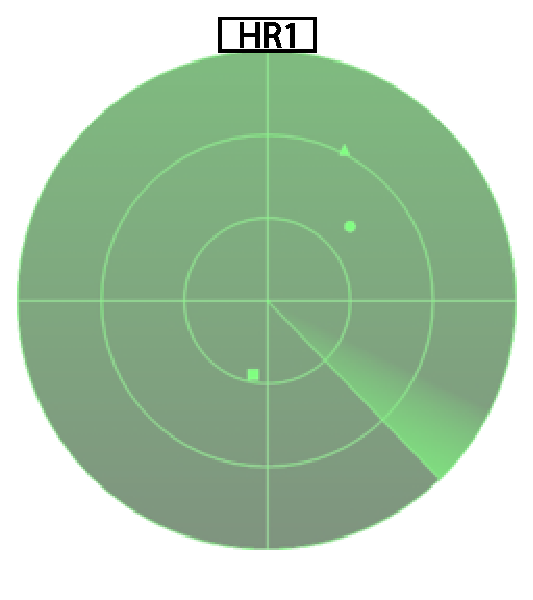
\includegraphics[width=\linewidth]{figure/radar1.eps}
    \caption{Mock up of inactive radar}
    \label{fig:mock_up_inactive_radar}
  \end{minipage}
  \hspace{0.5cm}
  \begin{minipage}[b]{0.5\linewidth}
    \centering
    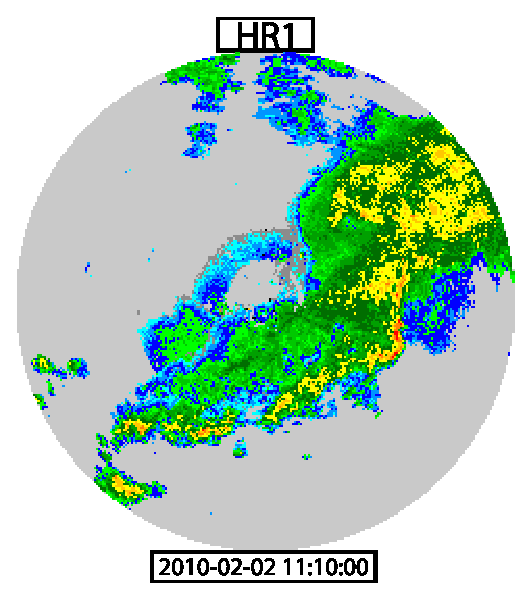
\includegraphics[width=\linewidth]{figure/radar2.eps}
    \caption{Mock up of active radar}
    \label{fig:mock_up_active_radar}
  \end{minipage}
\end{figure}
The added name and time stamp might pose as a problem, if two radars were placed in such a way that their range would overlap where the name or time stamp were put.

This could be somewhat solved, by fading out the radars too close to an active radar, in the same way that windmills inside the range of a radar is faded out when a radar animation starts.

\section{Data date range}
As time goes by, one would expect the application to contain massive amounts of data.
In the provided test data\footnote{Data02122.tar.gz provided by Pierre-Julien Trombe on CampusNet}, the application contains \textasciitilde 140 rows of data for \textsf{wrk} files and \textasciitilde 73,000 rows of data for the wind farm data.

It was discussed how we should limit the view of data, since it would require quite a lot of processing power to display that much data.

For the wind farm chart, we went from 1-month, weekly and daily view to 2-week, weekly and daily.
Preliminary tests showed that the loading time for 1-month view was too slow, because of the huge amount of data that had to be processed and formatted correctly before sent to the browser. The data would also take long to download, especially if not on a high speed internet connection.

Another problem was the radar images. Without any data range, they would all start at the first image taken by that radar, and play till the last. A range chosen by the user from a `to' and `from' date field was suggested. After testing the first implementation it was found that the `to' field was a bit confusing and would result in a bit of a rewrite of already existing code.

The `to' field was removed and the `from' field now decides the starting date for all radars and wind farm charts.
All radars will start their animation on the first image taken after the selected from date.
The chart will also start at the selected start date, but the navigation buttons allows one to go either back or forth in time independent of the selected from date.

\section{Radar interaction}
A lot of considerations went into the interaction of the radars. The primary focus of the radar design was to make it intuitive.

A `play' button to start animation of all radars were considered, but after a test implementation it was found to give a weird feeling and was removed again.

All radars will play after a single click and pause the animation if click while an animation is running. A double click will reset the radar to the first image and display the image for an inactive radar.

\section{The data}
\subsection{Implementation}
The massive amount of data forced a prioritized list of the order of which the data types should be implemented.

After a quick look at the data, it was decided that the data from the wind farm was the first one to be implemented due to its simplicity.

Research showed that the wrk file was in a relatively easy format with decent documentation\footnote{See \cite{VRIS} for the documentation}, where as the NetCDF\todo[color=red,fancyline]{foodnote / reference} format was very complex with little documentation\footnote{A framework for the file type was found but with very little documentation}.

After the implementation of wrk files, it was discussed whether or not the NetCDF should be implemented and it was decided that the time cost were too big to meet the deadline. Instead it was concluded that the flexibility of the application was good enough to allow extending the application to support other file formats, including NetCDF, at a later date and the focus was shifted to the frontend.

\subsection{Grouping wrk}
The big amount of wrk files for each radar (1 every \textasciitilde 10 minutes for a total of 144 files per day) causes a bit of confusion in the file administration of the control panel.

It was suggested that the administration panel grouped the wrk files per day, or that the data parser combined one day of wrk files into one file before importing it into the database.

The idea of letting the data parser to handle the merge was dropped due to the complexity. A merge in the data parser would also increase the memory usage by the data parser, which might not be available on the web server running the application.

Lack of time prevented the implementation of file grouping by the administration panel because of the work involved in finding the files that should be grouped together.

\subsection{Choice of map}
There were two obvious map options - Openstreetmap and Google maps. We know Google maps from Google, Facebook, etc.. The previous weather project were using Google maps, so at the beginning it was obvious that we were going to use Google maps.

\begin{figure}[htbp]
\begin{tabular}{| l | l | l |}
\hline
& \textbf{Openstreetmap} & \textbf{Google maps} \\
\hline
\textbf{Price} & Free & Free* \\
\hline
\textbf{View} & Standard & Standard, satellite and street view \\
\hline
\multirow{1}{*}{\textbf{License}} & Anyone can edit. & Owned by multiple organisations \\ & Open data (``CC BY-SA'') & and data is copyrighted (``NAVTEQ'' / ``TANA'') \\
\hline
\end{tabular}
\caption{Comparing Openstreetmap and Google maps}
\end{figure}
*Has a commercial price.

After comparing the two maps, it became quickly Openstreetmap. It was partly because of Google wants money if the map is used for commercial purposes and because the data is copyrighted and owned by multiple organisations. This wasn't the way we were thinking about open source.

Openstreetmap wasn't that difficult to work with, due to the very well documentation from leaflet\footnote{Documentations for openstreetmap - \url{http://leaflet.cloudmade.com}}\todo[color=red,fancyline]{move to references list?}.

\subsection{Frontend design}
\todo[inline]{More text}
There have been several design ideas. Many changes through the project and many considerations.
\subsubsection{Map}
\todo[inline]{reference to the figures throughout the section}
At the beginning we had a sidebar which could be visible or hidden. Later we found out that there is no need for a big menu, so we removed the sidebar and added a tiny top bar, with only the necessary options.\\
First mockup:
\begin{figure}[htbp]
   \centering
   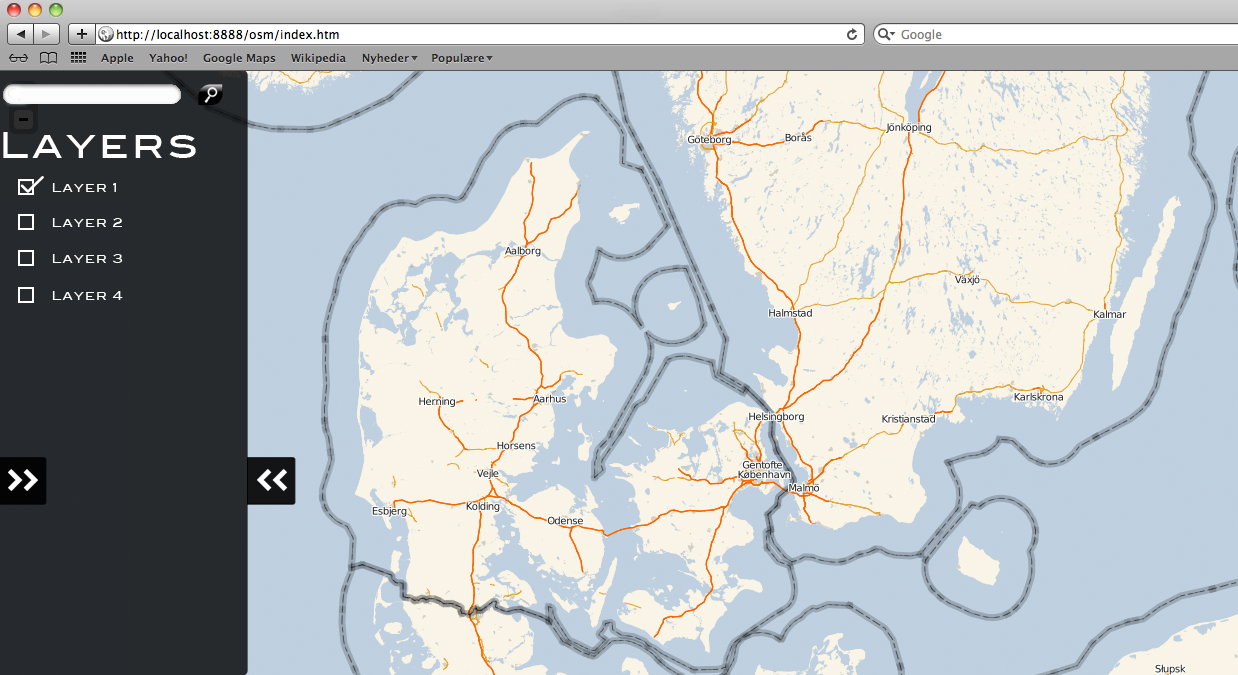
\includegraphics[scale=.3]{figure/design_map_v1.eps}
   \caption{Map - version 1}
\end{figure}

We would like to have different layers on the map at the beginning, but this was unnecessary, so it was quickly removed.\\
Now we have created a cool design which is easy to get used to and all relevant informations can be accessed easily and without to much clicking.
There have also been added some gestures to control the radar easily.\\
The top bar has a date field to know which date the radar should get data from. This date will be transferred to the chart window.

\begin{figure}[htbp]
   \centering
   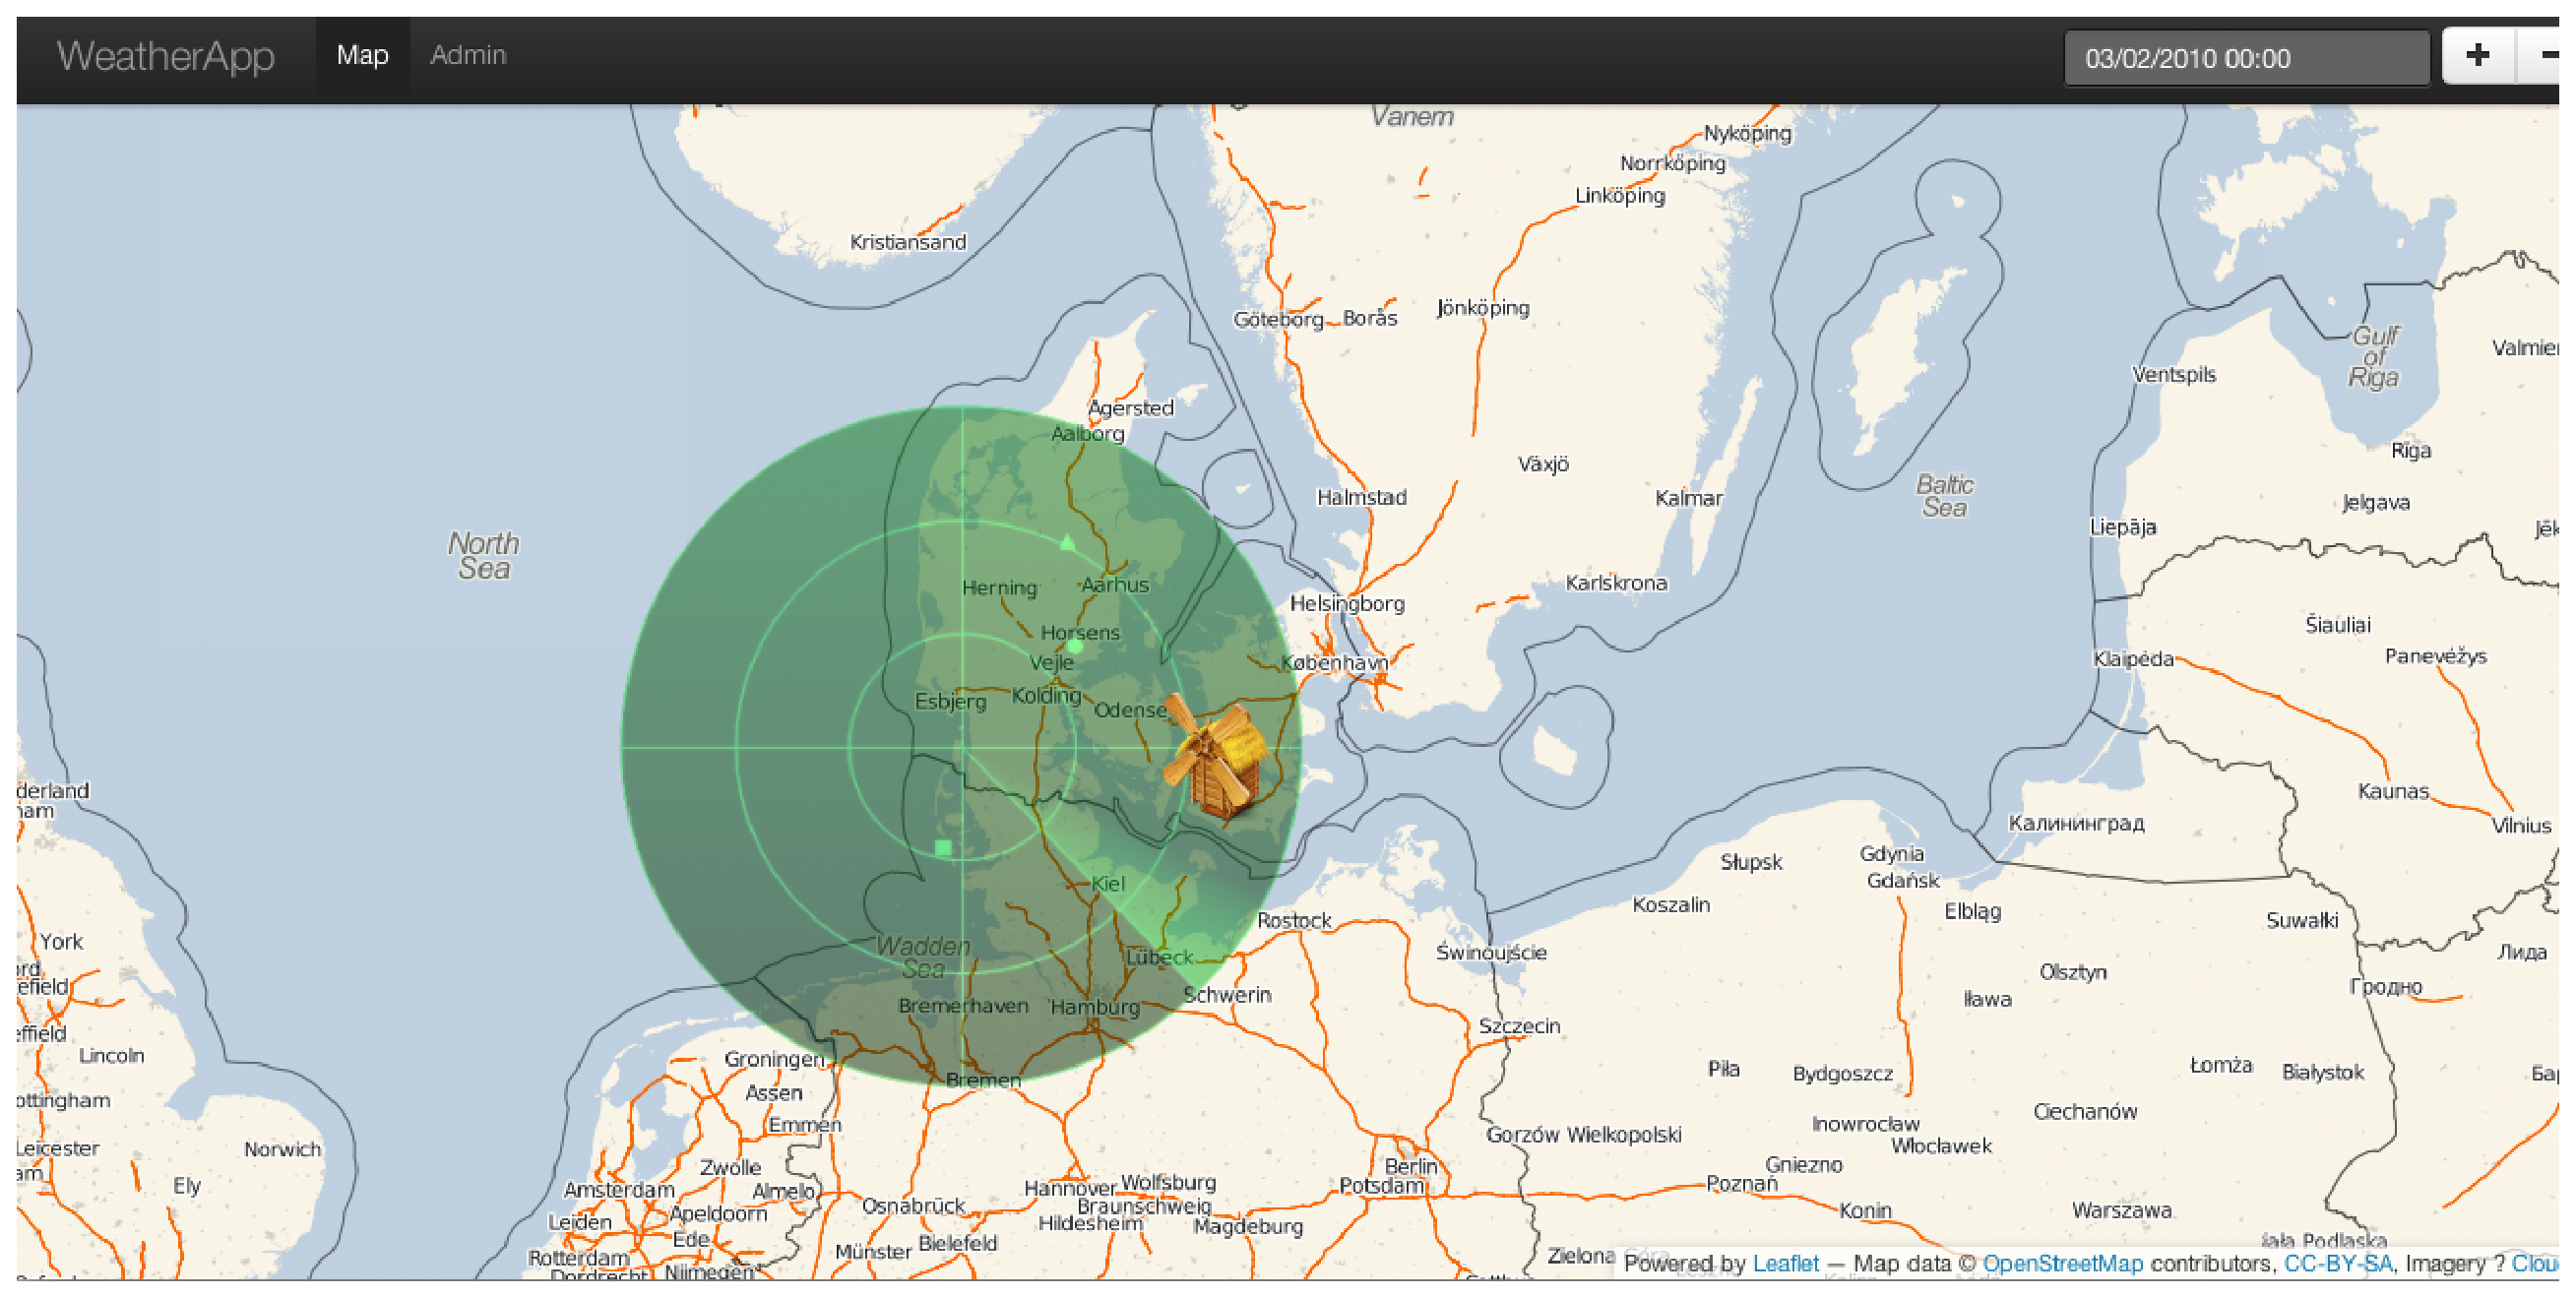
\includegraphics[width=1\linewidth]{figure/design_map_final.eps}
   \caption{Map - final}
\end{figure}

\subsubsection{Chart}
At the beginning we had the same sidebar as on the map, but with other options. This was also replaced by a top bar like on the map.\\
First mockup: 
\begin{figure}[htbp]
   \centering
   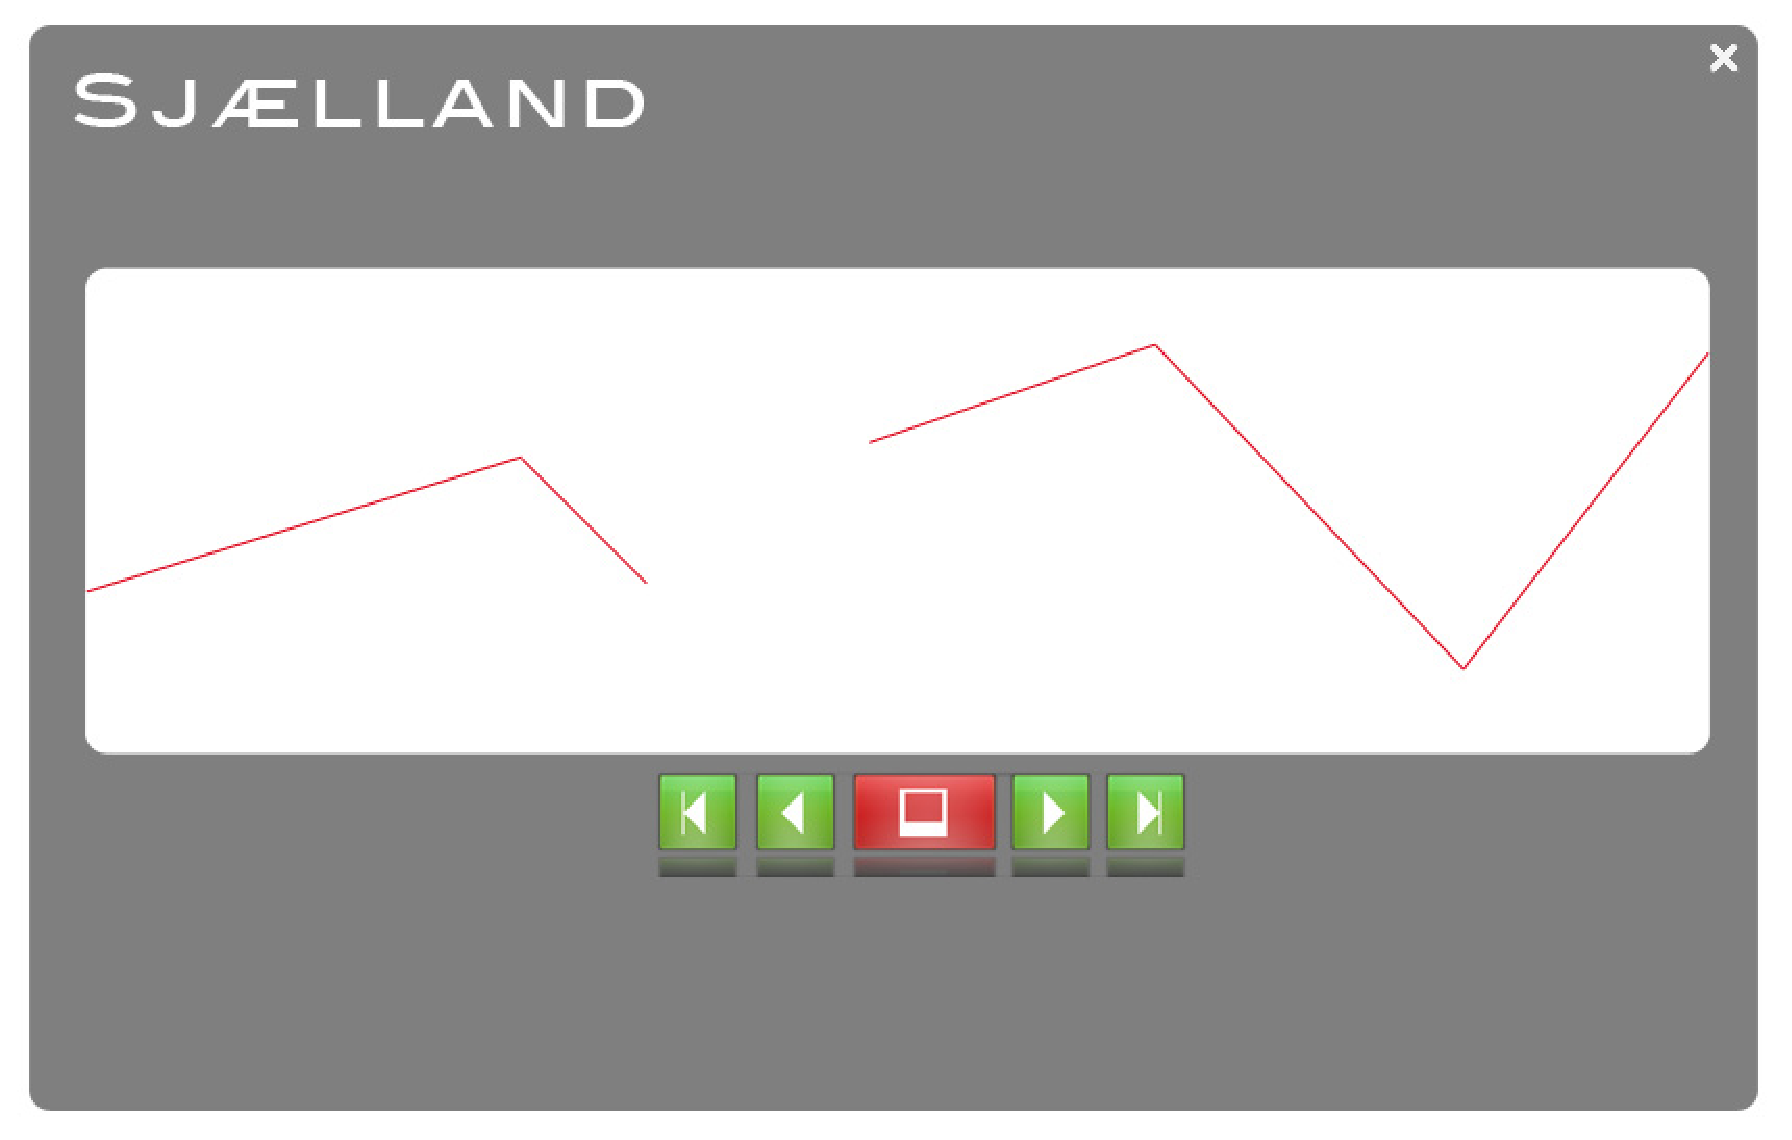
\includegraphics[width=1\linewidth]{figure/design_chart_v1.eps}
   \caption{Chart pop up - version 1}
\end{figure}

This has, through the whole project, been determined to be a pop up on the map.
The control buttons were before 'fast backward', 'backward', 'today', 'forward' and 'fast forward', but 'today' was replaced with 'play'. The 'play' button moves the chart every second, so the user can view the chart animated.\\
The new design also have three different views '2-week', 'weekly' and 'daily view'. Control buttons adjust to the view the user has selected.

\begin{figure}[htbp]
   \centering
   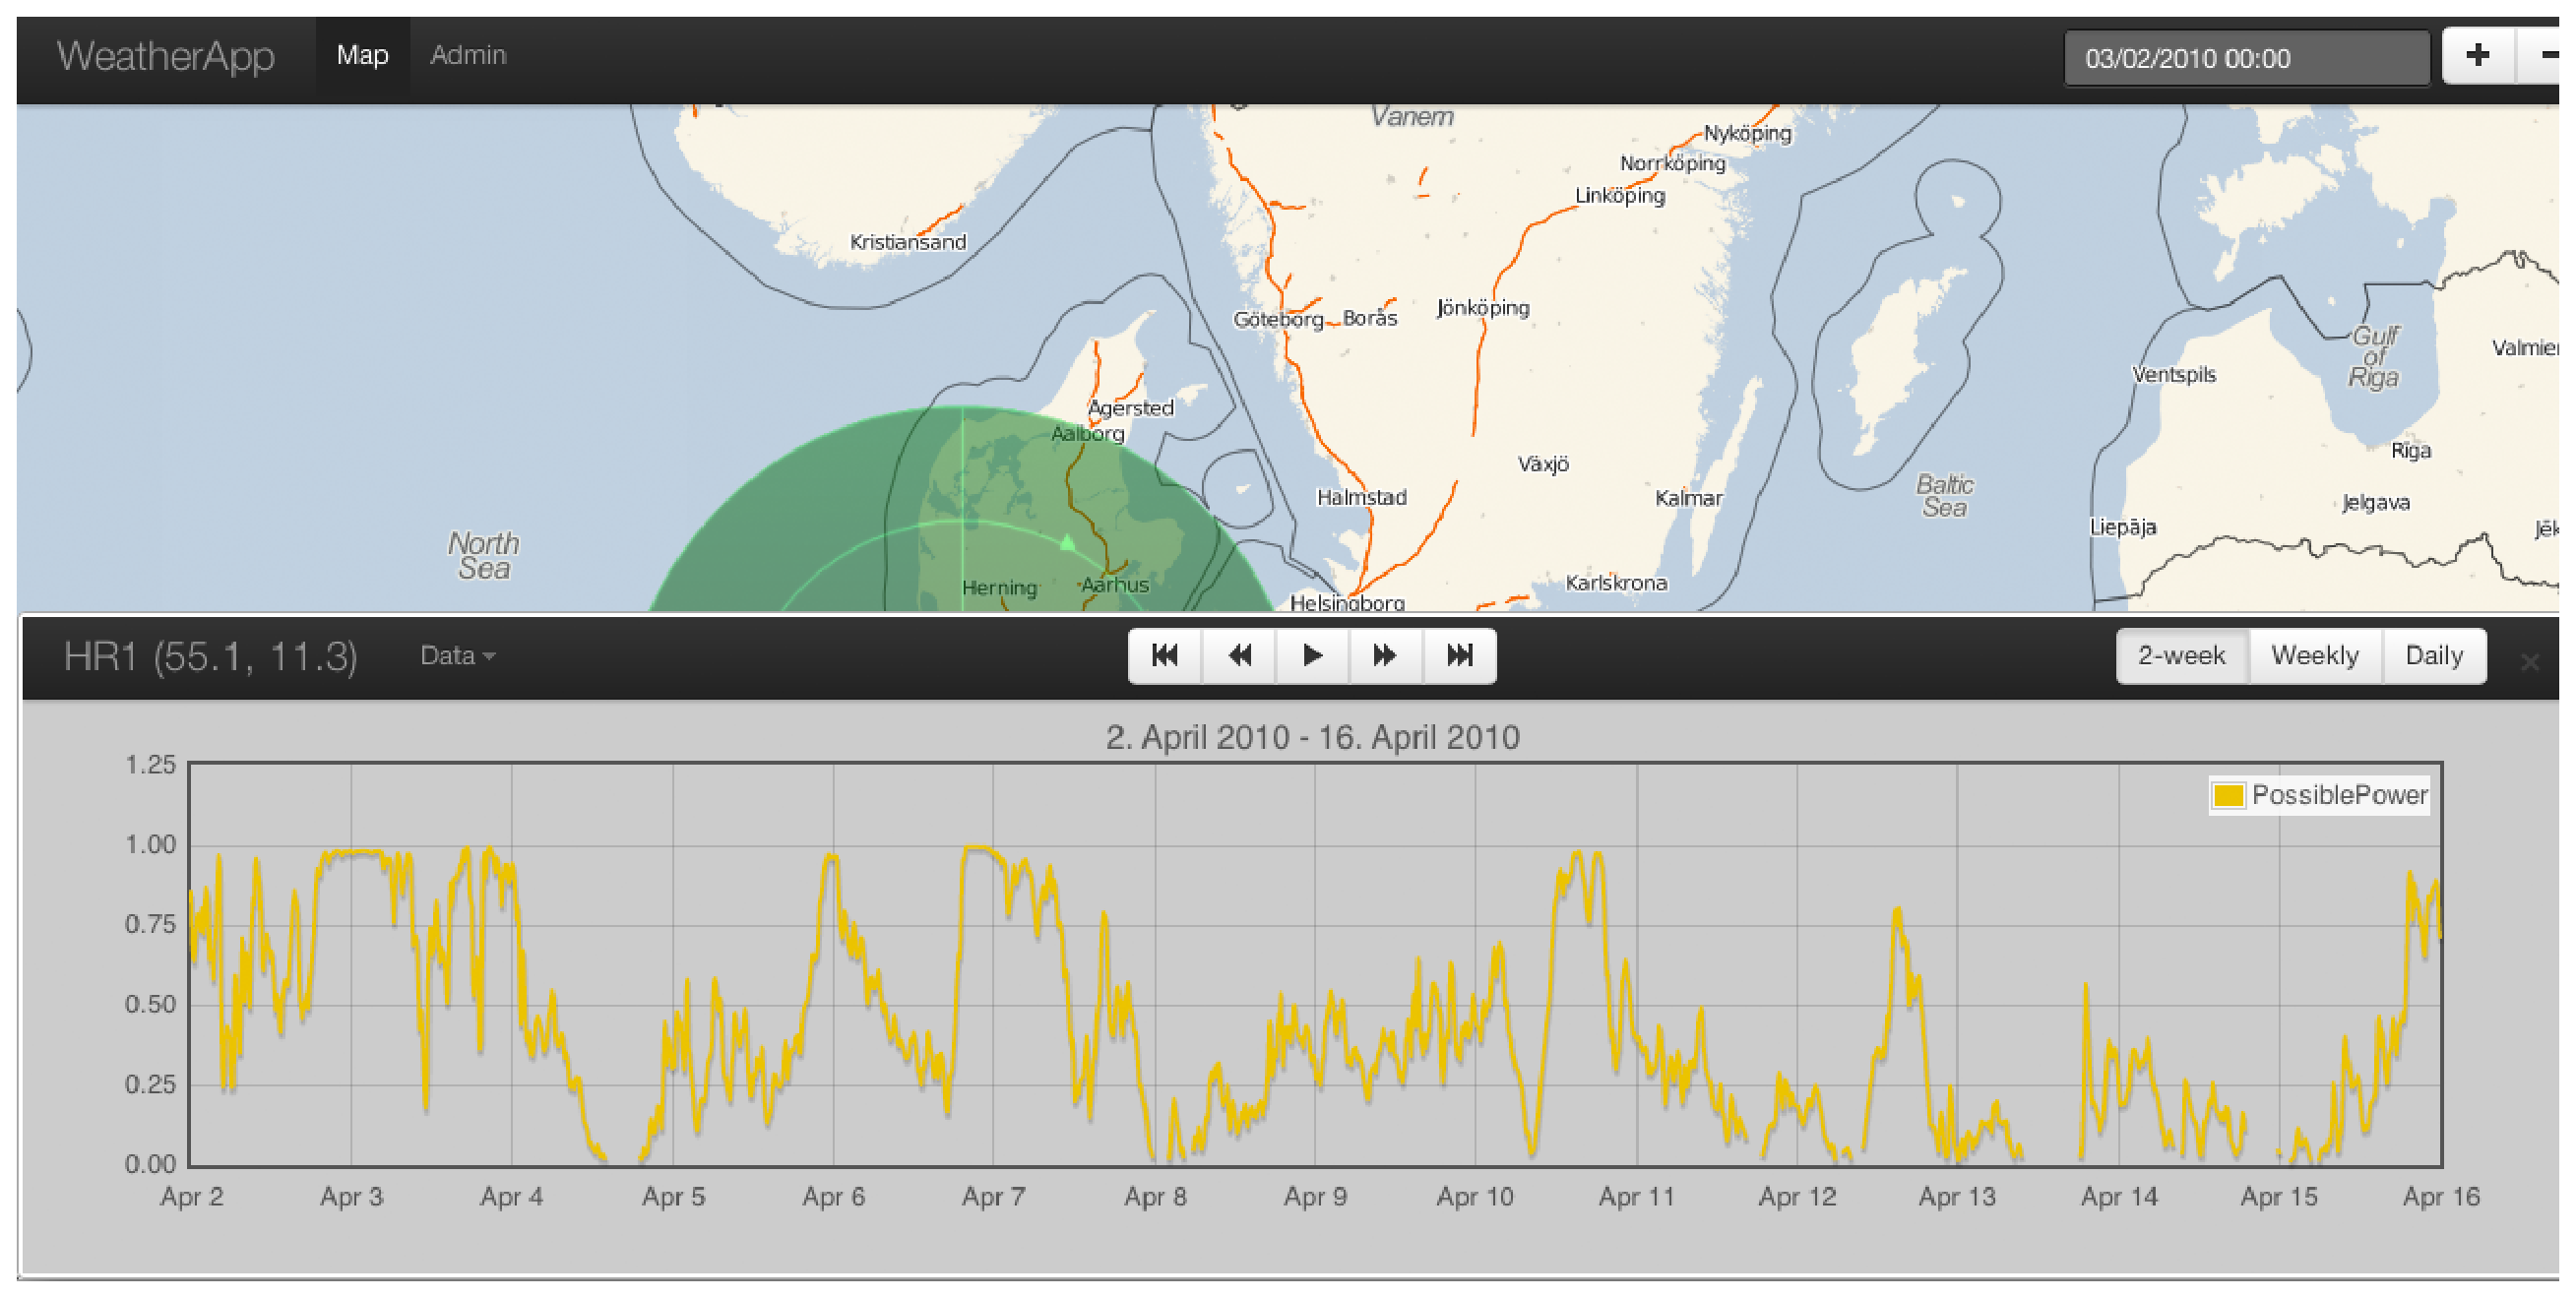
\includegraphics[width=1\linewidth]{figure/design_chart_final.eps}
   \caption{Chart pop up - final}
\end{figure}
